\documentclass[12pt]{article}
\usepackage{amsmath}
\usepackage{times}
\usepackage{hyperref}
\hypersetup{pdfpagemode=UseNone} % don't show bookmarks on initial view
\hypersetup{colorlinks, urlcolor={blue}}

% revise margins
\setlength{\headheight}{0.0in}
\setlength{\topmargin}{0.0in}
\setlength{\headsep}{0.0in}
\setlength{\textheight}{8.65in}
\setlength{\footskip}{0.35in}
\setlength{\oddsidemargin}{0.0in}
\setlength{\evensidemargin}{0.0in}
\setlength{\textwidth}{6.5in}

\setlength{\parskip}{6pt}
\setlength{\parindent}{0pt}

\usepackage{Sweave}
\begin{document}
\Sconcordance{concordance:p1partC01v02.tex:p1partC01v02.Rnw:%
1 20 1 1 0 16 1 1 11 13 0 1 3 3 1 1 10 6 0 1 2 3 1 2 2 36 1 1 12 13 0 1 %
3 4 1 1 10 6 0 1 3 3 1 1 2 1 3 40 1 1 10 11 0 1 2 3 1 1 9 6 0 1 2 2 1 1 %
2 1 3 9 1}


\sffamily \textbf{Assignment 1, TMA4300 Computer intenstive statistical methods}\\
{\sffamily \textbf{Student numbers: 750338, }}\\


{\sffamily \textbf{Problem A: Stochastic simulation by the probability integral transform}\\

{\sffamily \textbf{1) Exponential distribution}

One may use the the probability integral transform (PIT) to generate random samples from a exponential distribution. Given the cumulative distribution function
$F(x) = 1 - exp(-\lambda x)$ with rate $\lambda$, the inverse function is easily computed as $F^{-1}(F(x)) = -\frac{1}{\lambda}\log(1-f(x))$. Using
the PIT method an algorithm producing n samples is then given by:

\begin{figure}[H]
\centering
\begin{Schunk}
\begin{Sinput}
> expgenerator = function (lambda, n){
+ 
+   u = runif(n);
+ 
+   x = (-1/lambda)*log(1-u)
+ 
+ return(x)
+ 
+ }
> 
\end{Sinput}
\end{Schunk}
\end{figure}
In order to check if this is a proper generator:
\begin{figure}[H]
\centering
\begin{Schunk}
\begin{Soutput}
    rate 
1.917844 
\end{Soutput}
\end{Schunk}
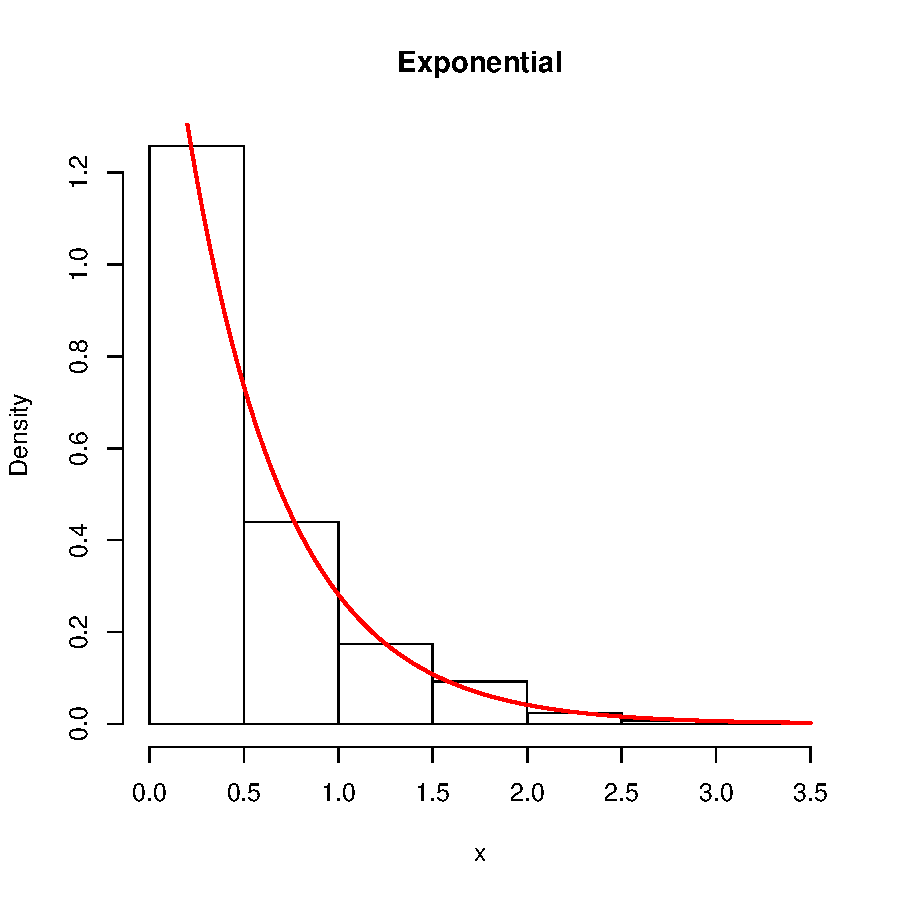
\includegraphics{p1partC01v02-002}
\end{figure}

\begin{figure}[H]
\centering
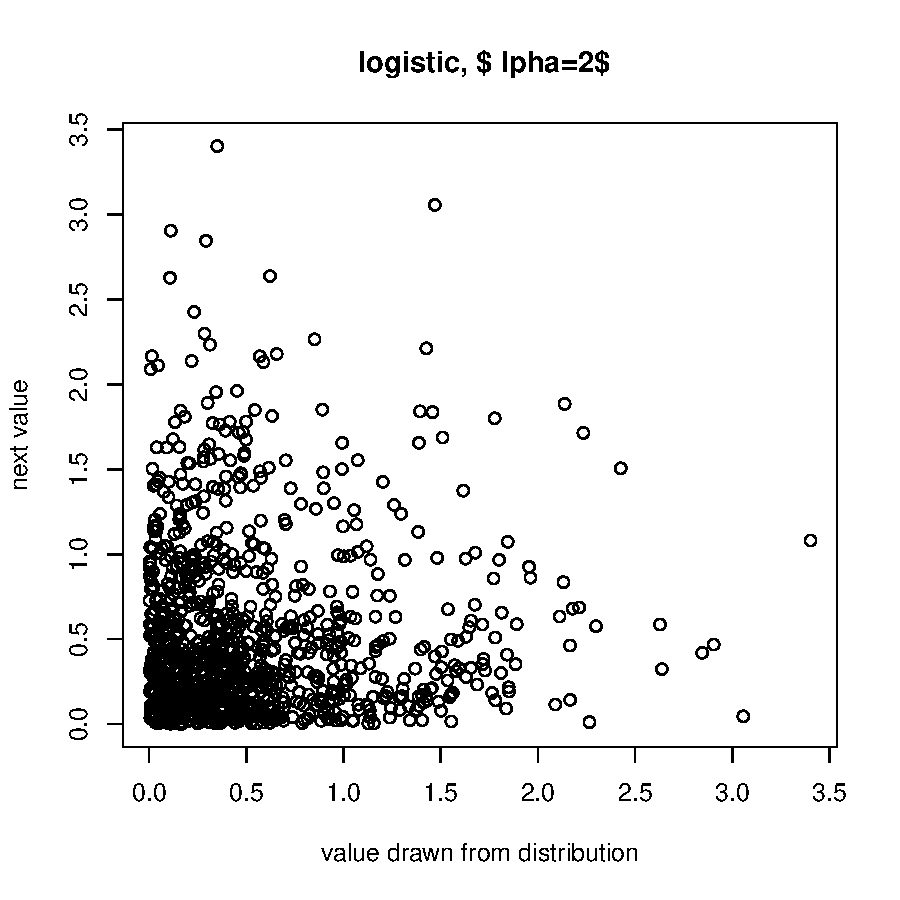
\includegraphics{p1partC01v02-003}
\end{figure}

{\sffamily \textbf{1) Another probability distribution}

Given the probability distribution:

\begin{equation}
f(x) = \frac{ce^{\alpha x}}{(1+e^{\alpha x})^2}, \quad -\infty < x < \infty, \quad \alpha >  0,
\end{equation}

where c is a normalizing constant. Integrating over the whole x-space, c must satisfy:

\begin{equation}
c \int_{-\infty}^{\infty} \frac{e^{\alpha x}}{(1+e^{\alpha x})^2} dx = \frac{c}{\alpha} \left[\frac{e^{\alpha x}}{1 + e^{\alpha x}}\right]_{-\infty}^{\infty} = \frac{c}{\alpha} = 1,
\end{equation}

which implies that $c = \alpha£$.

{\sffamily \textbf{Cumulative distribution and inverse function}

The cumulative distribution can now be found by definition

\begin{equation}
F(x) =  \alpha \int_{-\infty}^{x} \frac{e^{\alpha x'}}{(1+e^{\alpha x'})^2} dx' = \left[\frac{e^{\alpha x'}}{1 + e^{\alpha x'}}\right]_{-\infty}^{x} = \frac{e^{\alpha x}}{1+e^{\alpha x}}.
\end{equation}

The inverse function, $g(y)$, can easily be found by direct computation:

\begin{equation}
g(y) = \frac{1}{\alpha} \log{\frac{y}{1-y}}.
\end{equation}

In fact, this distribution is a logistic distribution with mean 0 and scale parameter, $\frac{1}{\alpha}$.
In order to generate samples from this distribution, the same method is used and the algorithm is given by:

\begin{figure}[H]
\centering
\begin{Schunk}
\begin{Sinput}
> logisticgenerator = function (alpha, n=1000){
+ 
+   u = runif(n);
+ 
+   x = (1/alpha)*log(u/(1-u))
+ 
+   return(x)
+ 
+ }
> 
\end{Sinput}
\end{Schunk}
\end{figure}
As before we chech how proper this generator is:

\begin{figure}[H]
\centering
\begin{Schunk}
\begin{Soutput}
   location       scale 
-0.02581635  0.51653561 
\end{Soutput}
\end{Schunk}
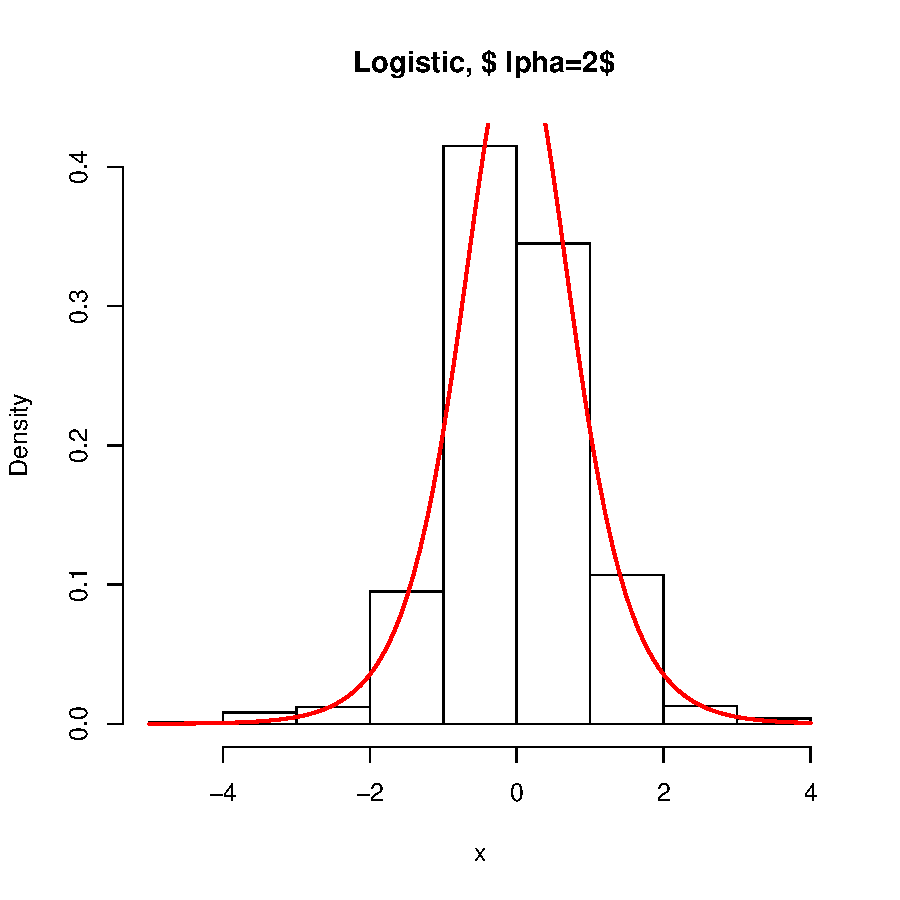
\includegraphics{p1partC01v02-005}
\end{figure}

\begin{figure}[H]
\centering
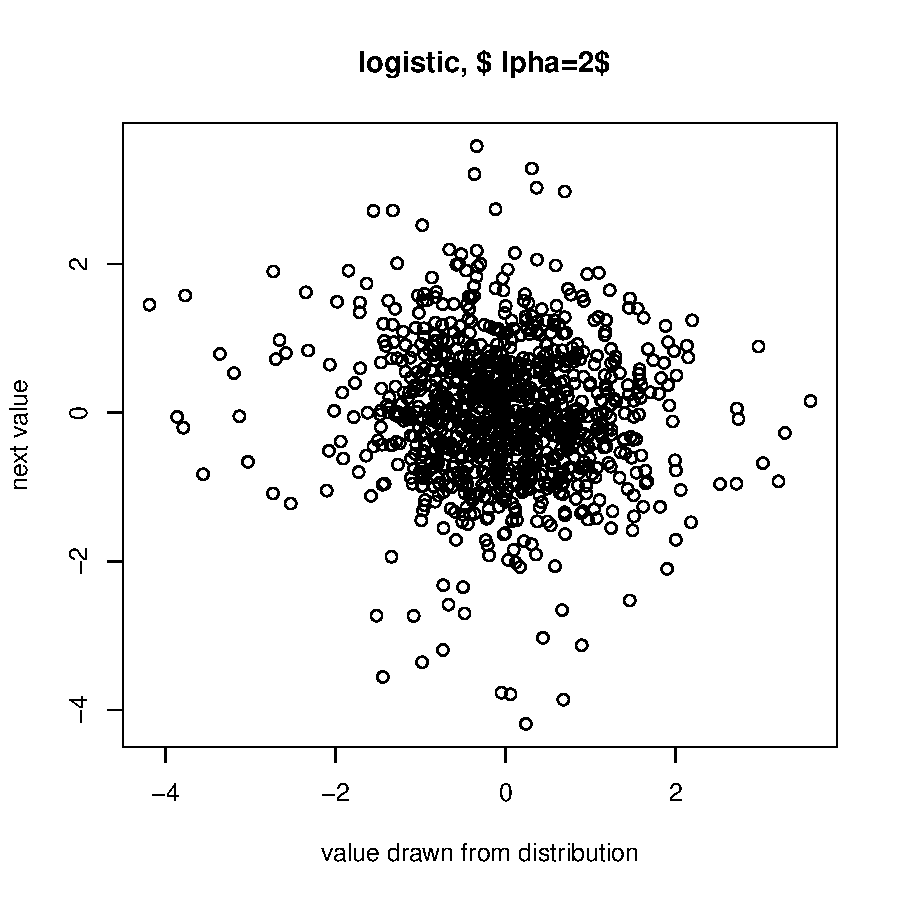
\includegraphics{p1partC01v02-006}
\end{figure}

{\sffamily \textbf{A3 - (a)}}
With probability density function
\begin{equation}
g(x) = \begin{cases} 
      0 & x\leq 0 \\
      c x^{\alpha-1} & 0 < x < 1 \\
      c e^{-x} & 1\leq x \\
   \end{cases}
\end{equation}
the cumulative distribution becomes
\begin{equation}
G(x) = \begin{cases} 
      0 & x\leq 0 \\
      \frac{c}{\alpha} x^{\alpha} & 0 < x < 1 \\
      \frac{c}{\alpha} + \frac{c}{e} - c e^{-x} & 1\leq x 
   \end{cases}
\end{equation}
and
\begin{equation}
1 = \lim_{x \to \infty} (\frac{c}{\alpha} + \frac{c}{e} - c e^{-x}) = c (\alpha^{-1}+e^{-1})
\end{equation}
such that $c = \frac{\alpha e}{e+\alpha}$. Since $G(1)=(1+e^{-1})^{-1}=0.731$ the inverse function will be defined differently beyond this point. The inverse function becomes
\begin{equation}
x = \begin{cases} 
      (\frac{c}{\alpha} G)^{\frac{1}{\alpha} & 0 < G < (1+e^{-1})^{-1} \\
      -log(1-G) + log(c) & (1+e^{-1})^{-1}\leq G +;.
   \end{cases}
\end{equation}
{\sffamily \textbf{A3 - (b)} recognizing the distribution and plotting it against the real thing.}

{\sffamily \textbf{C1 - (a)} Box-Muller algorithm for iid standard normal.}
The goal is to generate n independent samples from the standard normal distribution. The density of a standard normal distribution is
\begin{equation}
f(x)= \frac{1}{\sqrt{2\pi}} e^{\frac{x^2}{2}}
\end{equation}
plus some explanaition of why thhe algorithm work (find it in my notes which are at home).

\begin{figure}[H]
\centering
\begin{Schunk}
\begin{Sinput}
> stdnormalgenerator = function (n=1000){
+ 
+   u = 2*pi*runif(n/2)
+   x = expgenerator(1/2,n/2)
+   
+   return(c(sqrt(x)*sin(u), sqrt(x)*cos(u)))
+ 
+ } 
\end{Sinput}
\end{Schunk}
\end{figure}
and now we draw from it to check wether it behaves as expected
\begin{figure}[H]
\centering
\begin{Schunk}
\begin{Soutput}
         mean            sd 
-0.0009305537  1.0113502094 
\end{Soutput}
\end{Schunk}
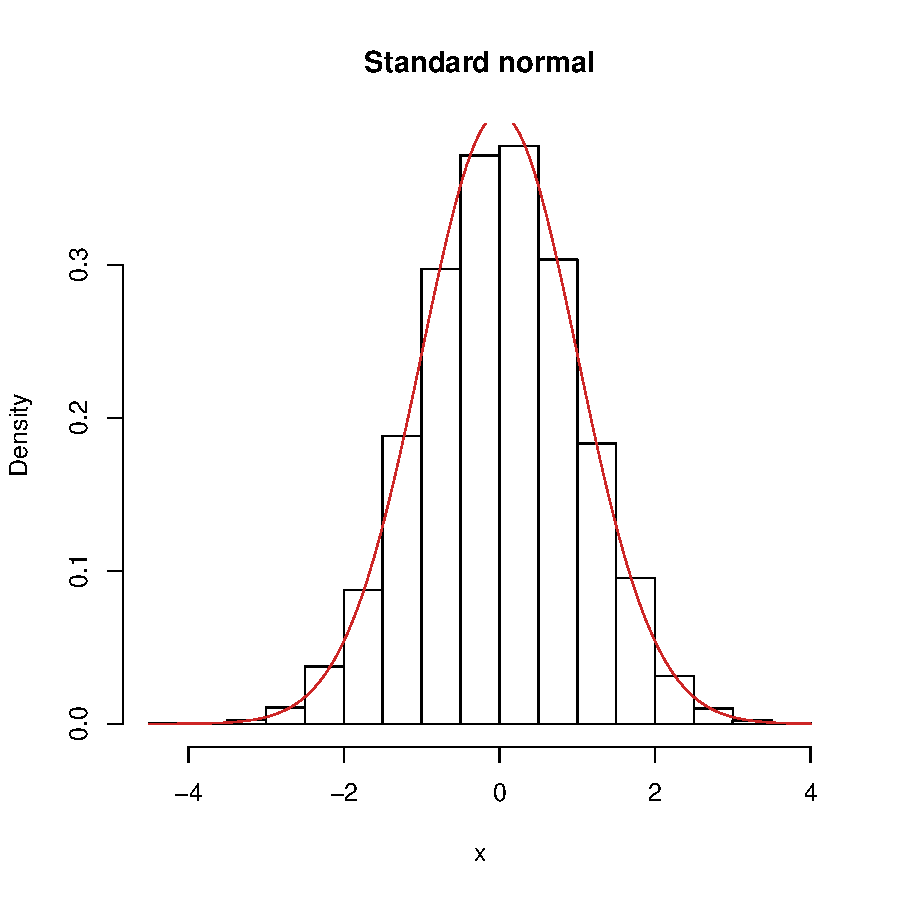
\includegraphics{p1partC01v02-008}
\end{figure}
\begin{figure}[H]
\centering
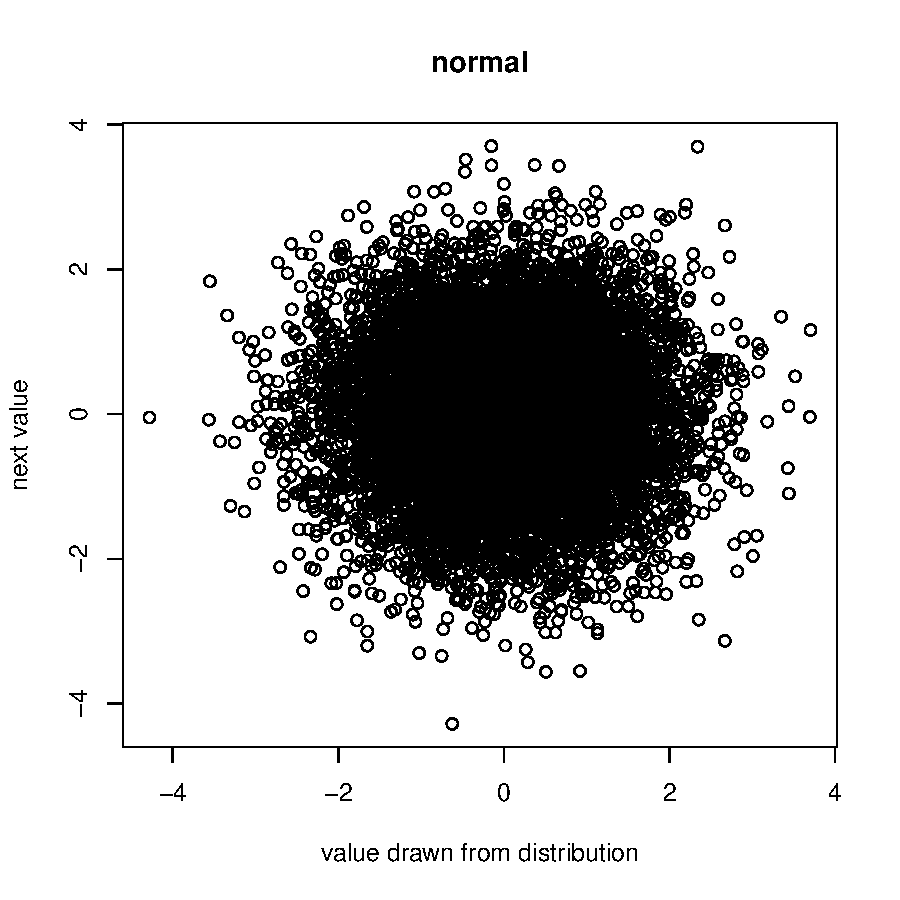
\includegraphics{p1partC01v02-009}
\end{figure}

\begin{thebibliography}{1}

\bibitem{Investopedia}
http://www.investopedia.com/articles/pf/10/credit-score-factors.asp

\end{thebibliography}

\end{document}
